\documentclass[sigconf]{acmart}

%% Class project: no ACM rights block / reference-format block
\setcopyright{none}
\settopmatter{printacmref=false}
\renewcommand\footnotetextcopyrightpermission[1]{}

%% Numbers below are generated by chess_baseline.py (upload the "out" folder next to this file)
\newcommand{\nRaw}{20{,}058}
\newcommand{\nGames}{19{,}113}
\newcommand{\nBinary}{18{,}225}
\newcommand{\nDraw}{888}
\newcommand{\pWhite}{49.9}
\newcommand{\pBlack}{45.4}
\newcommand{\pDraw}{4.6}
\newcommand{\ratingMin}{784}
\newcommand{\ratingMax}{2723}
\newcommand{\ratingMean}{1594}
\newcommand{\nOpenings}{365}
\newcommand{\nTrain}{14{,}580}
\newcommand{\nTest}{3{,}645}


\acmConference[CS-412]{CS-412 Machine Learning}{Fall 2026}{Chicago, IL, USA}\acmYear{2026}
\begin{document}

\title[Predicting Chess Outcomes]{Predicting Chess Game Outcomes from Pre-Game and Early-Game Features: A Comparison of Machine Learning Methods}
\subtitle{CS-412 Intermediate Project Report}

\author{Hashim Khan}
\affiliation{%
  \institution{University of Illinois Chicago}
  \city{Chicago}\state{Illinois}\country{USA}}

\renewcommand{\shortauthors}{Khan}

\begin{abstract}
This report describes progress on an application project that predicts the outcome of online chess games from player ratings, time control, and opening. Using \nGames{} Lichess games from Kaggle, we built a leakage-free preprocessing pipeline, defined a ``higher-rated player wins'' baseline, and trained five standard classifiers on a binary (White vs.\ Black) and a three-class (with draws) task. We summarize the data, the work completed so far, preliminary results, and the remaining plan for the final report.
\end{abstract}

\maketitle

\section{Introduction and Problem Description}
Chess is a two-player game with a large public record of games, and every game ends in a White win, a Black win, or a draw. Online platforms such as Lichess rate each player with a numerical rating that estimates playing strength, in the tradition of the Elo~\cite{elo} and Glicko~\cite{glicko} systems, which model win probability as a function of the rating difference. This project asks: \emph{how well can machine learning models predict the outcome of an online chess game from information available before or early in the game, and does a learned model improve on the simple rule that the higher-rated player wins?}

We study two prediction tasks on the same data. The \textbf{binary task} predicts whether White or Black wins and excludes draws. The \textbf{three-class task} also predicts draws, which are rare, so it additionally tests how models cope with class imbalance. We address three questions:
\begin{enumerate}
  \item Do machine learning models beat the baseline of ``the higher-rated player wins''?
  \item Which features matter most: ratings, opening, or time control?
  \item How does accuracy change as more of the game is revealed (e.g., the first 5 or 10 moves)?
\end{enumerate}
The first question has a preliminary answer in this report. Questions 2 and 3 require the feature-importance and early-move experiments described in Section~\ref{sec:remaining}.

A central methodological point is \textbf{data leakage}. Several columns in the raw data, such as how the game ended or how many moves it lasted, are only known after the game is over. A model using them would look accurate without being useful for prediction, so we exclude them (Section~\ref{sec:features}).

\section{Related Work}
Rating systems~\cite{elo,glicko} give a principled prediction from rating difference alone, which motivates our baseline. For tabular data like ours, tree ensembles such as Random Forests~\cite{breiman} and gradient boosting~\cite{xgboost} are standard strong methods, and a recent large benchmark found that tree-based models still outperform neural networks on medium-sized tabular datasets of about 10{,}000 samples~\cite{grinsztajn2022}. This is why we focus on classical models here. Deep learning has been applied to chess directly, as in DeepChess~\cite{deepchess} and AlphaZero~\cite{alphazero}, but those methods work on board positions and require far more data and compute. Our work instead compares standard classifiers on summary features, with explicit leakage control and a study of how much information early moves add.

\section{Data}
\subsection{Source and size}
We use the Lichess games dataset on Kaggle~\cite{kaggle}, which contains one row per game with player ratings, the time control, the opening, the full move list, and the result. The file has \nRaw{} rows. After removing duplicate game IDs and any rows with missing values or an invalid result (945 rows removed), \nGames{} games remain. Ratings range from \ratingMin{} to \ratingMax{} with a mean of \ratingMean{}. The games use \nOpenings{} distinct ECO opening codes.

\subsection{Target distribution}
Of the \nGames{} games, \pWhite\% are White wins, \pBlack\% are Black wins, and \pDraw\% (\nDraw{} games) are draws. The binary task therefore uses \nBinary{} games, and draws are a small minority class in the three-class task.

\subsection{Features and leakage control}\label{sec:features}
We use the following features, all available before the game starts or determined by its opening moves:
\begin{itemize}
  \item \texttt{white\_rating}, \texttt{black\_rating}, their difference, and their mean (we treat the recorded ratings as the players' ratings at the start of the game);
  \item time control: initial time in minutes and increment in seconds, parsed from \texttt{increment\_code};
  \item whether the game was rated;
  \item opening: the ECO letter (A--E), the 30 most frequent ECO codes (others grouped as ``other''), and \texttt{opening\_ply}.
\end{itemize}
We exclude \texttt{victory\_status} (how the game ended), \texttt{turns} (total number of moves), \texttt{created\_at} and \texttt{last\_move\_at} (their difference is the game duration), the full \texttt{moves} list (we will only use its first $N$ moves later), and the player IDs, which would let a model memorize individual players.

Table~\ref{tab:cols} summarizes how each raw column was handled.

\begin{table}[h]
  \caption{Handling of the raw columns.}
  \label{tab:cols}
  \footnotesize
  \begin{tabular}{@{}p{1.15in}p{0.6in}p{1.25in}@{}}
    \toprule
    Column(s) & Decision & Reason \\
    \midrule
    \texttt{white\_rating}, \texttt{black\_rating} & Use & Known before the game \\
    \texttt{increment\_code} & Use & Time control is fixed in advance \\
    \texttt{rated} & Use & Known before the game \\
    \texttt{opening\_eco}, \texttt{opening\_ply} & Use & Set by the first moves \\
    \texttt{victory\_status} & Exclude & Reveals how the game ended \\
    \texttt{turns} & Exclude & Game length is known only at the end \\
    \texttt{created\_at}, \texttt{last\_move\_at} & Exclude & Difference gives game duration \\
    \texttt{moves} & Later & Only the first $N$ moves will be used \\
    \texttt{id}, player IDs & Exclude & Identifiers; allow memorization \\
    \bottomrule
  \end{tabular}
\end{table}

\subsection{Exploratory analysis}
Figure~\ref{fig:winrate} shows White's win rate (draws excluded) as a function of the rating difference. White's win rate rises steadily from 17.7\% when Black is rated 300--400 points higher to 85.1\% when White is rated 300--400 points higher, so rating difference is a strong signal and the rating-based rule is a natural baseline.

\begin{figure}[t]
  \centering
  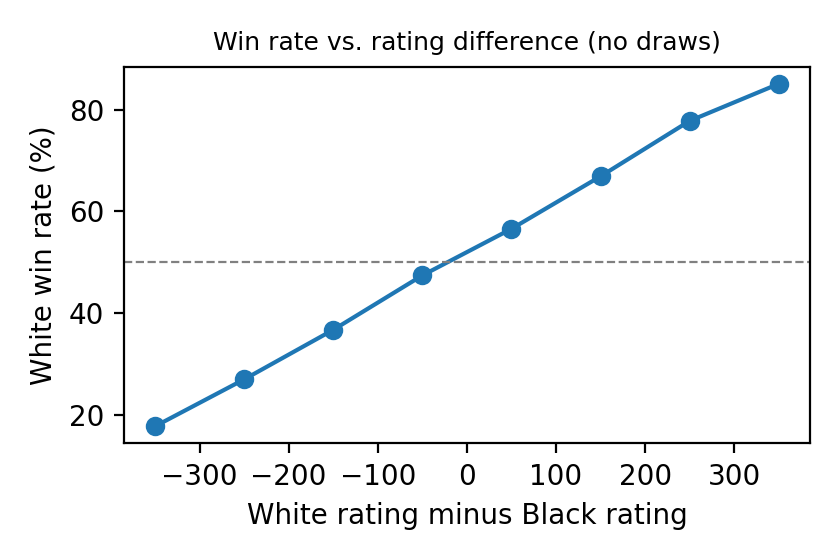
\includegraphics[width=0.95\linewidth]{out/winrate_by_ratingdiff.png}
  \caption{White's win rate by rating difference (White minus Black), in bins of 100 rating points, draws excluded.}
  \Description{Line plot of White's win rate in percent against rating difference.}
  \label{fig:winrate}
\end{figure}

\section{Work Completed So Far}
\subsection{Pipeline}
We implemented the full pipeline in a single Python script (\texttt{chess\_baseline.py}, in our GitHub repository) using pandas and scikit-learn. It loads and cleans the data, builds the features above, and splits the data into 80\% training and 20\% test sets, stratified by outcome with a fixed random seed. For the binary task this gives \nTrain{} training and \nTest{} test games. Numeric features are standardized and categorical features are one-hot encoded inside each model pipeline, so no information from the test set is used in preprocessing.

\subsection{Baselines and models}
We evaluate two baselines: always predicting the majority class, and predicting that the higher-rated player wins (White if the ratings are equal). We then train five classifiers with scikit-learn~\cite{sklearn}: Logistic Regression, a depth-5 Decision Tree, $k$-Nearest Neighbors ($k=25$), a Random Forest with 200 trees, and Gradient Boosting. These use mostly default settings; hyperparameter tuning is future work. Each model is evaluated by 5-fold cross-validation on the training set (accuracy, mean $\pm$ standard deviation) and then once on the held-out test set (accuracy and macro-averaged F1).

The models cover a range of complexity. \textbf{Logistic Regression} is a linear model whose predicted probability depends on a weighted sum of the features, and is a natural fit when the signal is mostly the rating difference. The \textbf{Decision Tree} splits the data with a sequence of threshold rules and is easy to interpret, but we limit its depth to 5 to avoid overfitting. \textbf{$k$-Nearest Neighbors} predicts from the 25 most similar training games, and is sensitive to how features are scaled, which is why numeric features are standardized. The \textbf{Random Forest}~\cite{breiman} averages many decorrelated trees, and \textbf{Gradient Boosting} builds trees one after another, each correcting the errors of the previous ones.

\subsection{Evaluation protocol}
We report accuracy, the fraction of games predicted correctly, because the binary task is nearly balanced. For the three-class task accuracy alone is misleading: since only \pDraw\% of games are draws, a model that never predicts a draw can still score well. We therefore also report \emph{macro-averaged F1}, which computes the F1 score of each class separately and averages them, so that the rare draw class counts as much as the two common classes. Cross-validation is stratified and run only on the training set; the test set is used once for the final numbers, so the reported test accuracy is not tuned to the test games.

\subsection{Preliminary results}
Table~\ref{tab:binary} reports the binary task and Table~\ref{tab:three} the three-class task. Figure~\ref{fig:acc} compares test accuracy on the binary task.

\begin{table}[t]
  \caption{Binary task (White vs.\ Black, draws excluded). Accuracy and macro-F1 in \%.}
  \label{tab:binary}
  \footnotesize
  \begin{tabular}{@{}p{1.35in}ccc@{}}
    \toprule
    Model & CV acc. & Test acc. & Test F1 \\
    \midrule
    Majority class & -- & 52.4 & 34.4 \\
Higher-rated player wins & -- & 65.2 & 65.2 \\
Logistic Regression & 65.0 $\pm$ 0.8 & 65.0 & 64.7 \\
Decision Tree (depth 5) & 64.8 $\pm$ 0.8 & 64.1 & 63.2 \\
k-NN (k=25) & 62.9 $\pm$ 0.7 & 63.3 & 63.0 \\
Random Forest (200 trees) & 63.1 $\pm$ 0.8 & 63.2 & 63.1 \\
Gradient Boosting & 65.1 $\pm$ 0.7 & 65.5 & 65.1%
\\
    \bottomrule
  \end{tabular}
\end{table}

\begin{table}[t]
  \caption{Three-class task (White, Black, draw). Accuracy and macro-F1 in \%.}
  \label{tab:three}
  \footnotesize
  \begin{tabular}{@{}p{1.35in}ccc@{}}
    \toprule
    Model & CV acc. & Test acc. & Test F1 \\
    \midrule
    Majority class & -- & 49.9 & 22.2 \\
Higher-rated player wins & -- & 62.3 & 42.5 \\
Logistic Regression & 61.9 $\pm$ 0.8 & 62.4 & 42.4 \\
Decision Tree (depth 5) & 61.7 $\pm$ 0.6 & 62.0 & 41.8 \\
k-NN (k=25) & 59.0 $\pm$ 1.4 & 60.0 & 40.9 \\
Random Forest (200 trees) & 60.3 $\pm$ 0.6 & 60.3 & 42.1 \\
Gradient Boosting & 61.4 $\pm$ 0.5 & 62.4 & 43.5%
\\
    \bottomrule
  \end{tabular}
\end{table}

\begin{figure}[t]
  \centering
  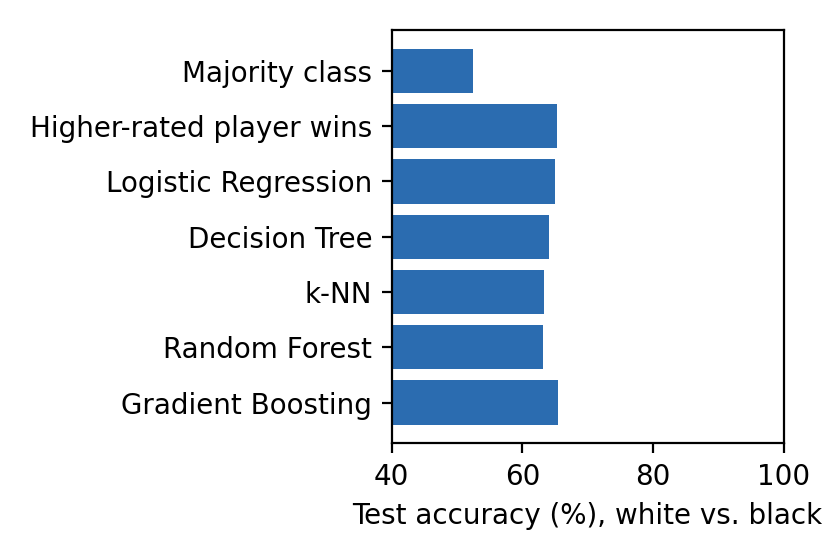
\includegraphics[width=0.95\linewidth]{out/model_accuracy.png}
  \caption{Test accuracy on the binary task for the baselines and the five models.}
  \Description{Horizontal bar chart of test accuracy for each model.}
  \label{fig:acc}
\end{figure}

None of the five models meaningfully improves on the rating-only rule. On the binary task the baseline reaches 65.2\% test accuracy, and the best models, Gradient Boosting (65.5\%) and Logistic Regression (65.0\%), are within a few tenths of a point of it, which is smaller than the cross-validation standard deviation of about 0.7--0.8 points. $k$-NN and the Random Forest are about two points lower (63.3\% and 63.2\%); a plausible reason is that the one-hot opening features, with hundreds of distinct opening codes, let these models fit noise, but we have not tested this yet. The three-class results are similar (baseline 62.3\%, Gradient Boosting 62.4\%). Macro-F1 is far below accuracy for every method (about 41--44\%) and close to the baseline's, which can never predict a draw, which suggests that the models also rarely identify draws; we will check per-class results. Overall, rating difference carries most of the usable signal, and the opening and time control appear to add little with default model settings. Whether tuning or early-move features change this is the focus of the remaining work.

\subsection{Challenges and lessons so far}
Three issues shaped the design. First, \textbf{leakage}: several raw columns would have made the models look far better than they are, so we audited every column before modeling (Table~\ref{tab:cols}). Second, \textbf{class imbalance}: draws make up only \pDraw\% of games, so plain accuracy is misleading in the three-class task, and we also report macro-F1. Third, \textbf{a strong baseline}: because the rating-only rule is already hard to beat, small differences between models are easy to over-interpret. We therefore compare differences against the cross-validation standard deviation.

\section{Remaining Work}\label{sec:remaining}
\begin{itemize}
  \item \textbf{Hyperparameter tuning} (Nov 2--12): cross-validated search over tree depth, number of trees, learning rate, and $k$, so that model comparisons are fair.
  \item \textbf{Early-move features} (Nov 13--20): extract the first $N$ moves (e.g., $N=5, 10$) from the move list and measure how much accuracy improves, which answers research question 3.
  \item \textbf{Feature importance and ablations} (Nov 13--20): measure which features matter, including a model without ratings to isolate the effect of the opening and time control.
  \item \textbf{Handling draws} (Nov 2--12): class weighting and per-class precision and recall for the three-class task.
  \item \textbf{Larger sample} (optional): a sample from the Lichess open database to check that conclusions hold at larger scale.
  \item \textbf{Presentation and final report}: presentation from mid-November; final 8--10 page report by Dec 1 (written Nov 21--30), with a clean repository.
\end{itemize}

Table~\ref{tab:status} summarizes the status of each project component against the milestones in the proposal.

\begin{table}[h]
  \caption{Project status against the proposal.}
  \label{tab:status}
  \footnotesize
  \begin{tabular}{@{}p{1.5in}p{1.4in}@{}}
    \toprule
    Component & Status \\
    \midrule
    Data download and cleaning & Done \\
    Leakage audit & Done \\
    Rating baseline and majority baseline & Done \\
    Five models, default settings & Done \\
    Binary and three-class evaluation & Done \\
    Hyperparameter tuning & Not started \\
    Feature importance and ablations & Not started \\
    Early-move features & Not started \\
    Final report and presentation & Not started \\
    \bottomrule
  \end{tabular}
\end{table}

\subsection{Risks}
The main risk is that the rating difference may remain by far the strongest feature, so tuning and extra features could add only small gains. This would not invalidate the project: showing carefully, with leakage control and a fair comparison, that a simple rule is hard to beat is itself a useful finding. If tuning gives no gain, the early-move experiment becomes the main contribution, since the first moves are the main information not yet used beyond ratings, opening, and time control. A second risk is dataset size: differences of a fraction of a point are within noise at about \nBinary{} games.

\section{Code and Team}
This is a solo project by Hashim Khan. All code, the proposal, and this report are maintained in the GitHub repository at \url{https://github.com/Hashimak03/Predicting-Chess-Game-Outcomes-ML-Project-}.

\bibliographystyle{ACM-Reference-Format}
\bibliography{references}

\end{document}
